\begin{frame}
  \frametitle{Unit Testing}

  \begin{itemize}
    \item **F**ast
    \item **I**solated
    \item **R**epetable 
    \item **S**elf-validating
    \item **T**imely
\end{itemize}

\end{frame}



\begin{frame}[fragile,shrink=30]
  \frametitle{Unit Tests}
  \framesubtitle{Unit Testing Using pytest}
  
  % what is unit testing

  The tests are performed through assertions:
  \begin{itemize}
    \item Whether or not the figure is generated
    \item The instance of the generated plot (a matplotlib figure, a plotly figure, etc.) 
    \item The writing of the generated figure in disk
  \end{itemize}

  \vspace{5mm}

  Example:
  \begin{lstlisting}[language=Python]
    v = Visualizer('/workspace/data/test_cc_3d.csv')
    fig = v.heatmap(title = 'This is a test heatmap',
                    xlabel = 'Countries', ylabel = 'Countries')
    assert fig.figure is not None
    assert isinstance(fig.figure, matplotlib.figure.Figure)
    fig.save('test_heatmap.png')
    assert Path('test_heatmap.png').is_file()
  \end{lstlisting}

  \begin{figure}[h]
    \centering
    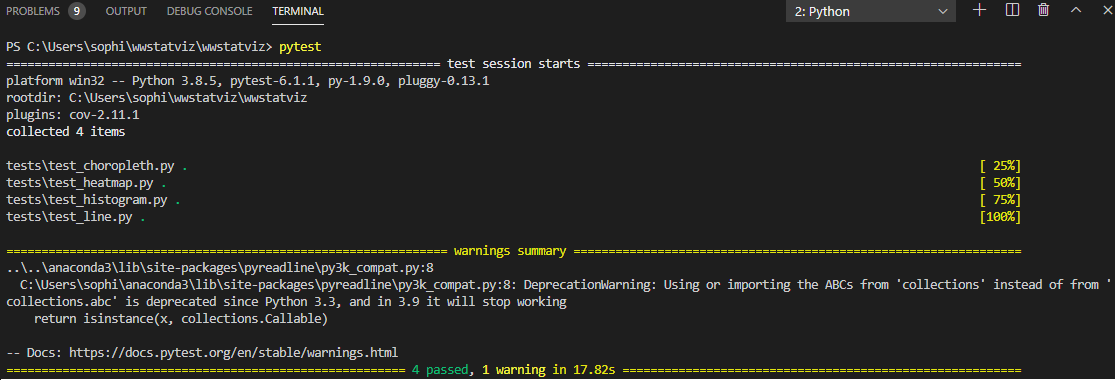
\includegraphics[scale=0.3]{tests.png}
    \caption{Unit Test Execution}
    \label{fig:tests}
  \end{figure}
  

\end{frame}
